\documentclass[main]{subfiles}

\begin{document}
    \subsection{(15.10.19) Практика совместно с 242 x2}

    \begin{Example}
      \[f: \R_+^* \times (0, 2\pi) \ra \R^3\]
      \[u,v \mapsto \Br{\dfrac{\cos v}{\ch u},\ \dfrac{\sin v}{\ch u},\ u - \th u}\]
      \begin{enumerate}
        \item Найдите $\RNumb{1}(F)$
        \item Найдите $\RNumb{2}(F)$
        \item Найдите кривизну Гаусса
        \item Найдите площадь поверхности
      \end{enumerate}
    \end{Example}

    \begin{Sol}
      \[\dfrac{\d f}{\d u} = \Br{-\dfrac{\cos v \sh u}{\ch^2 u},\ -\dfrac{\sin v \sh u}{\ch^2 u},\ \ob{= \th^2 u}{1 - \dfrac{1}{ch^2 u}}}\]
      \[\dfrac{\d f}{\d v} = \Br{-\dfrac{\sin v}{\ch u},\ \dfrac{\cos v}{\ch u},\ 0}\]
      \[<\dfrac{\d f}{\d u},\ \dfrac{\d f}{\d u}> = \th^2\]
      \[<\dfrac{\d f}{\d u},\ \dfrac{\d f}{\d v}> = 0\]
      \[<\dfrac{\d f}{\d v},\ \dfrac{\d f}{\d v}> = \dfrac{1}{\ch^2 u}\]
      \[\Ra \RNumb{1}(F) = \begin{pmatrix}
        {}\th^2 u & 0\\
        0 & \dfrac{1}{\ch^2 u}
      \end{pmatrix}\]
      \[\frac{\d F}{\d v} \times \frac{\d F}{\d u} =
      (
        -\cos v \dfrac{\th^2}{\ch u},\
        \sin \dfrac{\th^2 u}{\ch u},\
        -\dfrac{\sh u}{\ch^3 u}
      )\]
      \[\abs{\dfrac{\d F}{\d v} \times \dfrac{\d F}{\d u}} = \dfrac{\th u}{\ch u}\]
      \[n =
      \dfrac{
        \dfrac{\d F}{\d v} \times \dfrac{\d F}{\d u}
      }{
        \abs{\dfrac{\d F}{\d v} \times \dfrac{\d F}{\d u}}
      } = \Br{- \th u \cos v,\ -\th u \sin v,\ -\dfrac{1}{\ch u}}\]
      \[\frac{\d^2 F}{\d v^2} = \Br{-\dfrac{\cos v}{\ch u},\ -\dfrac{\sin v}{\ch u},\ 0}\]
      \[L = <\frac{\d^2 F}{\d v^2},\ \ol{n}> = -\dfrac{\sh u}{\ch^2 u}\]
      \[\frac{\d^2 F}{\d v \d u} = \Br{\dfrac{}{},\ \dfrac{}{},\ 0}\]
      \[M = <\frac{\d^2 F}{\d v \d u},\ \ol{n}> = 0\]
      \[\frac{\d^2 F}{\d u^2} = \Br{-\cos v \dfrac{1-\sh^2 u}{\ch^3 u},\ -\sin v \dfrac{}{}}\]
      \[N = <\frac{\d^2 F}{\d u^2},\ \ol{n}> = \dfrac{\sh u}{\ch^2 u}\]
      \[\Ra \RNumb{2}(F) = \begin{pmatrix}
        -\dfrac{\sh u}{\ch^2 u} u & 0\\
        0 & \dfrac{\sh u}{\ch^2 u}
      \end{pmatrix}\]

      \begin{figure}[H]
          %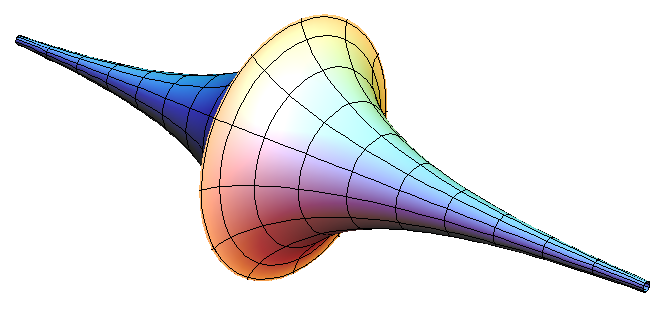
\includegraphics[scale=0.3]{pics/8_1}
          \centering
      \end{figure}

      \[A(S) = 2 \int_0^{\infty} \int_0^{2\pi} \dfrac{\sh u}{ch^2 u} du dv = 2 \cdot 2\pi \int_0^{\infty} \dfrac{\sh u}{\ch^2 u} du = 4\pi\]
    \end{Sol}

    \begin{Example}
      \[F: \R^2 \ra \R^3\]
      \[(u,v) \mapsto (F_1(u,v),\ F_2(u,v),\ F_3 (u,v))\]
      При каких условиях на $\RNumb{1}(F)$ F "сохраняет расстояние"\ (доказать)
    \end{Example}

    \begin{sol}
      %картинка
      \[l(\gamma) \os{?}{=} l (F \circ \gamma) = \int_0^1 \Abs{(F \circ \gamma)} dt\]
      \[\Ra \int^1_0 <\dot{\gamma}, \dot{\gamma}>^{\frac{1}{2}} dt \os{\forall \gamma}{=} \int_0^1 <\dot{\gamma}, \RNumb{1}(F) \dot{\gamma}> dt\]
      \[\text{т.к. }<\dot{\gamma}, \dot{\gamma}> = <\dot{\gamma}, \RNumb{1}(F) \dot{\gamma}>\q \forall \gamma\]
      \[\RNumb{1}(F) = \begin{pmatrix}
        a & b\\
        c & d
      \end{pmatrix} \text{ - ортогональная}\]
      \[\Ra \begin{cases}
        c=b\\
        a^2 + c^2 = 1\\
        b^2 + d^2 = 1\\
        ab + cd = 0\\
        ad - cb = \pm 1
      \end{cases}\]
      \[\text{т.к. $a,d > 0 \Ra$} \RNumb{1}(F) = \begin{pmatrix}
        1 & 0\\
        0 & 1
      \end{pmatrix}\]
    \end{sol}

    \begin{example}
      Сделаем цилиндр из плоскости с сохранением расстояния
      \[u,v \os{F}{\mapsto} (\cos v,\ \sin v,\ u)\]
      \[\RNumb{1}(F) = \begin{pmatrix}
        1 & 0\\
        0 & 1
      \end{pmatrix}\]
    \end{example}
\end{document}
